\section{Comparison with Experiments}\label{sec:validity}
\begin{figure}[t]
\centering
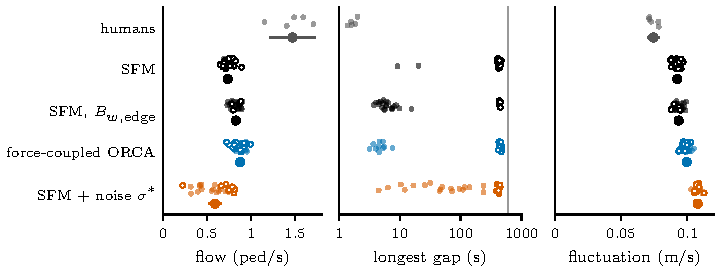
\includegraphics[width=\textwidth]{../figures/fig8_croma.pdf}
\caption{Flow, longest gap between passages (log scale; line, 600\,s horizon) and waiting-zone velocity fluctuation at the CroMa entrance ($w=0.8$\,m) for five human runs and 25 runs per model variant (squares, 2.0\,m corridor; circles, 0.2\,m), means and 95\% intervals as bars. Open markers: runs that did not complete; filled: completed runs.}
\label{fig:croma}
\end{figure}
% Table 3: outcomes of the CroMa model runs per variant (Sect. 8). Every number is a numbers.tex macro.
\begin{table}[t]
\caption{Outcomes of the 25 runs per model variant at the CroMa entrance.}
\label{tab:croma}
\centering\scriptsize\setlength{\tabcolsep}{3pt}
\begin{tabular*}{\textwidth}{@{\extracolsep{\fill}}lcccc@{}}
\toprule
Variant & Runs & Max.\ gap & Flow ratio [95\%] & No throttle [95\%]\\
\midrule
SFM & \RevDThreeCOneComplete/\RevDThreeCOneDeadlock/\RevDThreeCOneCapped & \PendCOneGapCompleteMax\,s & \RevDThreeCOneFlowRatio\ [\RevDThreeCOneFlowRatioLo, \RevDThreeCOneFlowRatioHi] & \RvBoneCroSfmRatio\ [\RvBoneCroSfmRatioLo, \RvBoneCroSfmRatioHi]\\
SFM, $B_{w,\rm edge}$ & \RevDThreeCEdgeComplete/\RevDThreeCEdgeDeadlock/\RevDThreeCEdgeCapped & \PendCEdgeGapCompleteMax\,s & \RevDThreeCEdgeFlowRatio\ [\RevDThreeCEdgeFlowRatioLo, \RevDThreeCEdgeFlowRatioHi] & \RvBoneCroEdgeRatio\ [\RvBoneCroEdgeRatioLo, \RvBoneCroEdgeRatioHi]\\
Force-coupled ORCA (RVO2) & \RevDThreeCThreeComplete/\RevDThreeCThreeDeadlock/\RevDThreeCThreeCapped & \PendCThreeGapCompleteMax\,s & \RevDThreeCThreeFlowRatio\ [\RevDThreeCThreeFlowRatioLo, \RevDThreeCThreeFlowRatioHi] & \RvBoneCroOrcaRatio\ [\RvBoneCroOrcaRatioLo, \RvBoneCroOrcaRatioHi]\\
SFM + noise $\sigma^\ast$ & \RevDThreeCSigComplete/\RevDThreeCSigDeadlock/\RevDThreeCSigCapped & \PendSigGapCompleteMax\,s & \RevDThreeCSigFlowRatio\ [\RevDThreeCSigFlowRatioLo, \RevDThreeCSigFlowRatioHi] & \RvBoneCroSigRatio\ [\RvBoneCroSigRatioLo, \RvBoneCroSigRatioHi]\\
\bottomrule
\end{tabular*}
\par\smallskip
\parbox{\textwidth}{\scriptsize Runs: complete/deadlock/still moving at 600\,s. Max.\ gap: longest gap of completed runs. No throttle: $v_{\rm eff}=v_0$, same spawns.}
\end{table}

%
\subsubsection{Experiments and Model Runs.}
The CroMa bottleneck experiments~\cite{fzj_ped20219,boomers2023data} include five laboratory runs through a 0.8\,m entrance. In two (4D030, 4D040) a corridor 2.0\,m long with thick tapered walls follows the entrance; the model represents these walls as thin. In three (4D110, 4D120, 4D130) the entrance is a door in a wall, 0.2\,m long. The runs mix three motivation conditions: participants walked normally (4D030, 4D110), hurried (4D040, 4D120) or gave full commitment (4D130). In all runs but 4D130 they kept a 2\,m semicircle before the entrance clear. The trajectories are published under CC BY 4.0~\cite{fzj_ped20219}; the experiments were approved by the ethics committee of the University of Wuppertal, and participants gave informed consent~\cite{boomers2023data}. All tracked participants pass, \RevDFourDonethirtyPassed--\RevDFourDthirtyPassed\ per run, and none deadlocks (duplicate track IDs merged).

As bottleneck flow grows with width~\cite{hoogendoorn2005,seyfried2009}, the model runs use the CroMa geometry and width (Sect.~\ref{sec:geometry}). Each human run has five model runs per variant, with as many agents as participants passed, starting at rest farther from the entrance than the participants and lasting up to 600\,s with uncalibrated default parameters. The four variants are SFM, SFM with the jamb range $B_{w,\rm edge}$, force-coupled ORCA and SFM with noise $\sigma^\ast$ (Sect.~\ref{sec:att-whole}). The model has no motivation parameter. Its mean agent diameter, \RvAnineModelDiameter\,m, is \RvAnineDiameterOverShoulder\ times the participants' mean shoulder width of \RvAnineShoulderWidth\,m (SD \RvAnineShoulderWidthSD\,m)~\cite{boomers2023data}.

A run's flow is $(N-1)/(t_N-t_1)$ for $N$ passages through the entrance plane at times $t_1\le\dots\le t_N$, counted up to any deadlock, so a model flow ratio is an upper bound on the flow of a run that deadlocks. The flow ratio of a variant is the mean flow of its 25 runs over the mean flow of the five human runs, with a 95\% interval from the log ratio (Welch $t$, unadjusted). The final gap of a run that deadlocks or still runs at 600\,s is right-censored. The velocity fluctuation is the SD of agents' velocities (smoothed as the humans') relative to neighbours within 0.74\,m, in the waiting zone (Fig.~\ref{fig:geometry}) while their mean speed is below 0.3\,m/s. The noise variant records no deadlock by its criterion, since noise keeps every agent's speed above 0.01\,m/s. Rerun at $\Delta t=0.005$\,s (25 runs per variant), every flow ratio lies inside its interval at 0.01\,s. In the noise variant at 0.01\,s bodies overlap by up to \RxCroSigFullOverlapM\,m, and the explicit friction step exceeds its stability bound of 2 in \RxCroSigFullFrictionRunsGeTwo\ of 25 runs (factor $2\kappa h\Delta t/m=\RzMiscFrictionOne$, $h$ the largest overlap; \RzMiscFrictionHalf\ at 0.005\,s).

%
\subsubsection{Flow and Passage Gaps.}
Between the 10\% and the 90\% passage, which every run reaches, the variants pass \RvAnineWindowRatioMin--\RvAnineWindowRatioMax\ of the human flow. Over whole runs human flow is \PendHumanFlow\ [\PendHumanFlowLo, \PendHumanFlowHi]\,ped/s, and the fastest model run (\PendModelFlowMax\,ped/s) is slower than the slowest human run (\PendHumanFlowMin\,ped/s). The human runs mix three motivation levels and two geometries, so the comparison tests the order of the model flow at uncalibrated defaults. The longest human gap averages \EtenHumanGap\,s (maximum \EtenHumanGapMax\,s at 0.01\,s resolution); \EtenHumanGapsOverTwoTotal\ gap in the five runs exceeds 2\,s.

Model passages come in bursts: \PendCThreeGapsTwo--\PendSigGapsTwo\ gaps longer than 2\,s per run (Fig.~\ref{fig:croma}, Table~\ref{tab:croma}). The Kaplan--Meier median longest gap is \RevDThreeCEdgeGapKMMedian\,s (jamb range) and \PendSigGapKMMedian\,s (noise), at least \PendCOneGapLowerMedianTwo\ and \PendCThreeGapLowerMedianTwo\,s for SFM and force-coupled ORCA. Model velocity fluctuation (\RevDThreeCOneFluct--\RevDThreeCSigFluct\,m/s) exceeds the human one, \EtenHumanFluct\ [\EtenHumanFluctLo, \EtenHumanFluctHi]\,m/s. With uncalibrated defaults the variants pass \RevDThreeRatioMin--\RevDThreeRatioMax\ of the human flow over whole runs. The density throttle of Eq.~\eqref{eq:des} lowers the desired speed in this dense passage; without it every ratio rises but stays below 1 (\RvBoneCroOffMin--\RvBoneCroOffMax, same spawns; Table~\ref{tab:croma}).
